\chapter{阅读亲缘关系：系统发生树}\label{ch:g12:phylogenetic-trees}

1837 年，达尔文在一本私人笔记本的一页上画了一条分枝线，
线上连着几根小枝，并在其上方写下两个词：“我想”。这幅草图
提出，\omterm{def:g10:biodiversity-scales:species}{物种}之间的亲缘关系如同树枝之间的关系一样——
即由共同的主枝分化而来——并且这种亲缘关系可以被重建。
如今，这幅草图已是一种标准工具：\omterm{def:g12:phylogenetic-trees:tree}{系统发生树}，
由共有性状和 \omterm{def:g10:universal-dna:information}{DNA} 构建，并依据一定规则进行判读。
本章讲授这些规则：如何由性状表构建树，
如何读懂树而不致误读，以及分子如何
使它变成一把“分子钟”。

\section{树说明了什么}

\begin{definition}[系统发生树]\label{def:g12:phylogenetic-trees:tree}
\emph{系统发生树}\index{系统发生树}是一种图示，
表示一组\omterm{def:g10:biodiversity-scales:species}{物种}（或其他类群）之间的亲缘关系。其枝端是
所比较的\omterm{def:g10:biodiversity-scales:species}{物种}；每个两条分支相交的\emph{节点}代表
它们最近的共同祖先——一个假想的\omterm{def:g12:selection-drift-speciation:population}{种群}，而非已知的
化石；\emph{根}是所有\omterm{def:g10:biodiversity-scales:species}{物种}的共同祖先。两个\omterm{def:g10:biodiversity-scales:species}{物种}比
第三者更近缘，是指它们的共同祖先（即它们的节点）
比它们与第三者共有的节点更近。亲缘关系应由节点读取，
绝不能由枝端的左右位置读取。
\end{definition}

\begin{proposition}[阅读规则]\label{prop:g12:phylogenetic-trees:rules}
\begin{itemize}
  \item 树可在任一节点处旋转而不改变其
        含义：枝端的顺序是任意的。
  \item 节点没有名称，也不是枝端之一：一个\omterm{def:g10:biodiversity-scales:species}{物种}
        绝不是树上另一\omterm{def:g10:biodiversity-scales:species}{物种}的祖先；两个枝端
        互为\emph{姐妹群}，源自同一共同祖先。
  \item 由一个祖先及其\emph{全部}后代组成的类群——
        即一个节点之后的全部成员——是\emph{演化支}\index{演化支}，
        是系统发生分类唯一命名的类群。
  \item 只有树图作了说明时，分支长度才携带信息
        （时间或变化次数）；否则
        只有分支顺序有意义。
\end{itemize}
\end{proposition}
\admitted

\begin{omfigure}
\begin{tikzpicture}[font=\small, line cap=round]
  % tree 1
  \begin{scope}
    \draw[thick] (0,0) -- (1,0);
    \draw[thick] (1,0) -- (1,1.2) -- (4.5,1.2);
    \draw[thick] (1,0) -- (1,-1.2) -- (2.2,-1.2);
    \draw[thick] (2.2,-1.2) -- (2.2,-0.5) -- (4.5,-0.5);
    \draw[thick] (2.2,-1.2) -- (2.2,-1.9) -- (3.4,-1.9);
    \draw[thick] (3.4,-1.9) -- (3.4,-1.5) -- (4.5,-1.5);
    \draw[thick] (3.4,-1.9) -- (3.4,-2.3) -- (4.5,-2.3);
    \node[anchor=west] at (4.6,1.2) {青蛙}; \node[anchor=west] at (4.6,-0.5) {蜥蜴};
    \node[anchor=west] at (4.6,-1.5) {小鼠}; \node[anchor=west] at (4.6,-2.3) {人类};
    \fill[omThm] (1,0) circle (2pt); \fill[omThm] (2.2,-1.2) circle (2pt); \fill[omThm] (3.4,-1.9) circle (2pt);
    \node[anchor=north, align=center] at (2.8,-2.7) {树 A};
  \end{scope}
  % tree 2: same topology, rotated
  \begin{scope}[xshift=8cm]
    \draw[thick] (0,0) -- (1,0);
    \draw[thick] (1,0) -- (1,1.2) -- (2.2,1.2);
    \draw[thick] (2.2,1.2) -- (2.2,1.9) -- (3.4,1.9);
    \draw[thick] (3.4,1.9) -- (3.4,2.3) -- (4.5,2.3);
    \draw[thick] (3.4,1.9) -- (3.4,1.5) -- (4.5,1.5);
    \draw[thick] (2.2,1.2) -- (2.2,0.5) -- (4.5,0.5);
    \draw[thick] (1,0) -- (1,-1.2) -- (4.5,-1.2);
    \node[anchor=west] at (4.6,2.3) {人类}; \node[anchor=west] at (4.6,1.5) {小鼠};
    \node[anchor=west] at (4.6,0.5) {蜥蜴}; \node[anchor=west] at (4.6,-1.2) {青蛙};
    \fill[omThm] (1,0) circle (2pt); \fill[omThm] (2.2,1.2) circle (2pt); \fill[omThm] (3.4,1.9) circle (2pt);
    \node[anchor=north, align=center] at (2.8,-2.7) {树 B：同一棵树};
  \end{scope}
\end{tikzpicture}

{\small 同一棵树的两幅图。在每个节点处旋转分支
只改变枝端的顺序，而不改变任何亲缘关系：两图中，
小鼠与人互为姐妹群，蜥蜴是它们最近的亲属，而
青蛙的亲缘关系最远。由图 A 读出“蜥蜴位于青蛙
与小鼠之间”便是错误的。}
\end{omfigure}

\begin{example}[应避免的误读]\label{ex:g12:phylogenetic-trees:misreadings}
“人类由黑猩猩进化而来”：不对——树上，人与黑猩猩
互为姐妹枝端，源自一个共同祖先，该祖先
两者都不是。“青蛙更原始”：不对——每个枝端都是现存\omterm{def:g10:biodiversity-scales:species}{物种}，
自根部起的演化历史长度相同；青蛙谱系
与我们的谱系演化了同样长的时间。“蜥蜴与青蛙的
亲缘关系比与小鼠更近”（由图 A 得出）：不对——蜥蜴与小鼠
共有一个更近的节点。
\end{example}

\section{由性状构建树}

\begin{definition}[祖先状态与衍生状态]\label{def:g12:phylogenetic-trees:states}
\emph{性状}是指在所比较的\omterm{def:g10:biodiversity-scales:species}{物种}之间存在差异的特征
（如是否有脊柱、是否有四肢、是否有羊膜卵，
是否有毛发）。每个性状都有一种\emph{祖先状态}——
即该类群共同祖先所具有的状态——以及一种或多种\emph{衍生状态}，
这些状态在某些谱系中较晚出现。只有\emph{共有衍生状态}
才能指示亲缘关系：共有同一衍生状态的两个\omterm{def:g10:biodiversity-scales:species}{物种}，是从
产生该状态的祖先那里继承了它。共有祖先状态
并不能说明任何问题，因为所有\omterm{def:g10:biodiversity-scales:species}{物种}的祖先都具有它。
\end{definition}

\begin{method}[由性状矩阵到树]\label{met:g12:phylogenetic-trees:build}
\begin{enumerate}
  \item 制作一张表：行为\omterm{def:g10:biodiversity-scales:species}{物种}，列为性状，衍生状态记为 1，
        祖先状态记为 0。判定哪种状态是祖先状态，需与
        \emph{外群}比较，外群是
        已知位于所研究类群之外的\omterm{def:g10:biodiversity-scales:species}{物种}。
  \item 找出被最多\omterm{def:g10:biodiversity-scales:species}{物种}所共有的衍生状态：它界定
        第一个、也是最大的\omterm{prop:g12:phylogenetic-trees:rules}{演化支}。在其内部，再找
        下一个共有范围最广的衍生状态，依此类推。
  \item 将嵌套的\omterm{prop:g12:phylogenetic-trees:rules}{演化支}画成树：每一个共有衍生状态
        标出一个节点，该性状则标在它出现的
        分支上。
  \item 检查冲突：某性状为一些\omterm{def:g10:biodiversity-scales:species}{物种}所共有，但其他性状却把它们分开，
        则该性状要么是两次独立产生（趋同），要么曾丢失一次。
        应选择在全部性状上所需变化次数最少的树——
        即最\emph{简约}的树。
\end{enumerate}
\end{method}

\begin{omfigure}
\begin{tikzpicture}[font=\small, line cap=round]
  % matrix
  \node[anchor=east] at (-0.2,2.4) {};
  \matrix (m) [matrix of nodes, nodes={font=\small, minimum width=1.1cm, minimum height=0.5cm, anchor=center},
               column 1/.style={nodes={anchor=east, minimum width=1.6cm}}] at (1.6,0.5) {
    \phantom{o} & 颌 & 四肢 & 羊膜 & 毛发 \\
    七鳃鳗 & 0 & 0 & 0 & 0 \\
    鳟鱼 & 1 & 0 & 0 & 0 \\
    蛙 & 1 & 1 & 0 & 0 \\
    蜥蜴 & 1 & 1 & 1 & 0 \\
    小鼠 & 1 & 1 & 1 & 1 \\
  };
  \draw (m-1-1.south west) -- (m-1-5.south east);
  \draw (m-1-2.north west) -- (m-6-2.south west);
  % tree
  \begin{scope}[xshift=7.2cm, yshift=-1.4cm]
    \draw[thick] (0,0) -- (0.8,0);
    \draw[thick] (0.8,0) -- (0.8,3.2) -- (5,3.2);
    \draw[thick] (0.8,0) -- (0.8,-0.6) -- (1.8,-0.6);
    \draw[thick] (1.8,-0.6) -- (1.8,2.4) -- (5,2.4);
    \draw[thick] (1.8,-0.6) -- (1.8,-1.0) -- (2.8,-1.0);
    \draw[thick] (2.8,-1.0) -- (2.8,1.6) -- (5,1.6);
    \draw[thick] (2.8,-1.0) -- (2.8,-1.3) -- (3.8,-1.3);
    \draw[thick] (3.8,-1.3) -- (3.8,0.8) -- (5,0.8);
    \draw[thick] (3.8,-1.3) -- (3.8,-1.5) -- (5,-1.5);
    \node[anchor=west] at (5.1,3.2) {七鳃鳗}; \node[anchor=west] at (5.1,2.4) {鳟鱼};
    \node[anchor=west] at (5.1,1.6) {青蛙}; \node[anchor=west] at (5.1,0.8) {蜥蜴};
    \node[anchor=west] at (5.1,-1.5) {小鼠};
    \foreach \x/\y/\t in {1.3/-0.6/颌, 2.3/-1.0/四肢, 3.3/-1.3/羊膜, 4.4/-1.5/毛发}
      { \draw[very thick, omThm] (\x,\y+0.15) -- (\x,\y-0.15); \node[font=\scriptsize, omThm, anchor=north] at (\x,\y-0.2) {\t}; }
    \node[anchor=east, font=\scriptsize] at (-0.1,0) {外群：七鳃鳗};
  \end{scope}
\end{tikzpicture}

{\small 由矩阵画树。一组\omterm{def:g10:biodiversity-scales:species}{物种}所共有的每个衍生状态（1）
标出它们共同祖先的节点；红色竖线标出各性状出现的位置。
七鳃鳗缺少全部衍生状态，它作为外群，用以确定
祖先状态。}
\end{omfigure}

\begin{example}[用简约原则解决的冲突]\label{ex:g12:phylogenetic-trees:parsimony}
在由蝙蝠、鸽子和小鼠组成的矩阵中加入“翅膀”一项。“翅膀”会把蝙蝠与鸽子归为一类；
毛发和乳汁则把蝙蝠与小鼠归为一类。若使蝙蝠与小鼠聚在一起，
则翅膀需两次独立产生（共两次变化）；若使蝙蝠与鸽子聚在一起，
则毛发、乳汁、哺乳动物的颌及其他十多个性状都需各自两次独立产生。
第一种树远为简约：翅膀是趋同产生的，
哺乳动物的各项性状则为共同继承。简约性并不能证明
系统树是否正确，它只是选出
其中最不可能有误的那一棵。
\end{example}

\section{由分子构建系统树}

\begin{proposition}[分子系统发生]\label{prop:g12:phylogenetic-trees:molecular}
被比较的所有\omterm{def:g10:biodiversity-scales:species}{物种}所共有的一个\omterm{def:g10:universal-dna:gene}{基因}或\omterm{def:g11:gene-expression:protein}{蛋白质}本身就是一个性状矩阵：
序列中的每个位点是一个性状，
每个\omterm{def:g10:universal-dna:nucleotide}{核苷酸}或\omterm{def:g10:chemistry-of-life:families}{氨基酸}是一个状态。将序列比对，
并计算每一对之间的差异，即得到距离矩阵，
再由此按先合并最近一对的方式构建树。
由与解剖学无关的序列计算得到的分子树，
在绝大多数情况下与解剖学树相吻合——
这是对二者最有力的检验。
\end{proposition}
\begin{proof}[证据]
在\cref{ch:g10:common-ancestry}中给出了
\omterm{def:g10:common-ancestry:bodyplan}{脊椎动物}\omterm{def:g10:cells-common-unit:cell}{细胞}色素 c 的距离，这些距离重现了依据骨骼所绘的分支图。
在灵长类中，数十个\omterm{def:g10:universal-dna:gene}{基因}的序列相互印证：人与
黑猩猩的 \omterm{def:g10:universal-dna:information}{DNA} 相差约 1.2\%，人与大猩猩相差
1.6\%，三者与红毛猩猩相差 3\%，大型类人猿与
猕猴相差 7\%。由其中任一\omterm{def:g10:universal-dna:gene}{基因}构建的树形状相同；
少数例外涉及最近的节点，
那里的差异最小。
\end{proof}

\begin{omfigure}
\begin{tikzpicture}[font=\small, line cap=round]
  \draw[thick] (0,0) -- (1,0);
  \draw[thick] (1,0) -- (1,2.4) -- (8,2.4);
  \draw[thick] (1,0) -- (1,-0.8) -- (3,-0.8);
  \draw[thick] (3,-0.8) -- (3,1.2) -- (8,1.2);
  \draw[thick] (3,-0.8) -- (3,-1.4) -- (5.2,-1.4);
  \draw[thick] (5.2,-1.4) -- (5.2,0) -- (8,0);
  \draw[thick] (5.2,-1.4) -- (5.2,-2.0) -- (6.4,-2.0);
  \draw[thick] (6.4,-2.0) -- (6.4,-1.2) -- (8,-1.2);
  \draw[thick] (6.4,-2.0) -- (6.4,-2.8) -- (8,-2.8);
  \node[anchor=west] at (8.1,2.4) {猕猴}; \node[anchor=west] at (8.1,1.2) {红毛猩猩};
  \node[anchor=west] at (8.1,0) {大猩猩}; \node[anchor=west] at (8.1,-1.2) {黑猩猩};
  \node[anchor=west] at (8.1,-2.8) {人};
  \foreach \x/\t in {1/{25}, 3/{14}, 5.2/{9}, 6.4/{6}}
    { \fill[omThm] (\x,-3.4) circle (0); \node[font=\scriptsize, omThm, anchor=north] at (\x,-3.4) {\t}; \draw[gray, dashed] (\x,-3.3) -- (\x,-3.0); }
  \draw[->, gray] (0.5,-3.5) -- (8,-3.5) node[midway, below=7pt, font=\scriptsize] {百万年前（节点年代由分子钟与化石确定）};
  \node[font=\scriptsize, anchor=south] at (7.2,-1.05) {DNA 差异 1.2\%};
  \node[font=\scriptsize, anchor=south] at (6.6,0.15) {1.6\%};
  \node[font=\scriptsize, anchor=south] at (5.5,1.35) {3\%};
  \node[font=\scriptsize, anchor=south] at (4.5,2.55) {DNA 相差 7\%};
\end{tikzpicture}

{\small 由 \omterm{def:g10:universal-dna:information}{DNA} 比较得到的五种灵长类的系统树。人与
黑猩猩互为姐妹类群；大猩猩随后并入，再依次为红毛猩猩和猕猴。
每一分支上的百分数为其所连接两个\omterm{def:g10:biodiversity-scales:species}{物种}之间的 \omterm{def:g10:universal-dna:information}{DNA}
差异；下方的年代来自由化石校准的
分子钟。}
\end{omfigure}

\begin{proposition}[分子钟]\label{prop:g12:phylogenetic-trees:clock}
对于某一给定\omterm{def:g10:universal-dna:gene}{基因}，两条谱系之间的差异在长时间内
以大致恒定的速率累积，因为多数替换是中性的，
并以其产生的速率经漂变而固定。两个\omterm{def:g10:biodiversity-scales:species}{物种}之间的
差异数因此与它们自共同祖先以来的时间成正比。
若以一个由化石定年的节点校准，分子钟便可推定
其余节点的年代——但须注意，速率在不同\omterm{def:g10:universal-dna:gene}{基因}和
不同谱系之间各不相同，且校准本身也带有
不确定度。
\end{proposition}
\admitted

\begin{omfigure}
\begin{tikzpicture}
\begin{axis}[
  width=0.84\linewidth, height=5.6cm,
  axis x line=bottom, axis y line=left,
  xmin=0, xmax=30, ymin=0, ymax=8,
  xlabel={距共同祖先的时间（百万年，由化石测定）},
  ylabel={DNA 差异（\%）},
  xlabel style={font=\small, at={(axis description cs:0.5,-0.12)}, anchor=north},
  ylabel style={font=\small},
  tick label style={font=\small}, xtick={0,5,10,15,20,25,30}, ytick={0,2,4,6,8},
  clip=false,
]
\addplot[only marks, mark=*, mark size=2pt, omThm] coordinates {(6,1.2) (9,1.6) (14,3.0) (25,7.0)};
\addplot[thick, omDef, domain=0:28] {0.27*x};
\node[font=\scriptsize, anchor=west] at (axis cs:6.4,1.0) {人–黑猩猩};
\node[font=\scriptsize, anchor=west] at (axis cs:9.4,1.5) {--大猩猩};
\node[font=\scriptsize, anchor=west] at (axis cs:14.4,2.9) {--猩猩};
\node[font=\scriptsize, anchor=east] at (axis cs:24.6,7.1) {--猕猴};
\end{axis}
\end{tikzpicture}

{\small 灵长类的分子钟：\omterm{def:g10:universal-dna:information}{DNA} 差异随共同祖先
的年龄而变化。各点近似落在一条直线上，斜率约为
每百万年 0.27\%；该直线可用于由 \omterm{def:g10:universal-dna:information}{DNA} 差异推定
无化石节点的年代。}
\end{omfigure}

\begin{example}[定年节点]\label{ex:g12:phylogenetic-trees:dating}
两个\omterm{def:g10:biodiversity-scales:species}{物种}的 \omterm{def:g10:universal-dna:information}{DNA} 相差 4.5\%；按每百万年 0.27\% 计，
它们的共同祖先约生活在 1700 万年前。该估计
假定适用灵长类的速率；若某\omterm{def:g10:universal-dna:gene}{基因}的进化速度快一倍，
或位于世代较短的谱系中，相同的 4.5\% 则意味着
时间便只有一半。分子钟的可靠程度取决于其校准。
\end{example}

\section{由树看分类}

\begin{proposition}[按谱系分类]\label{prop:g12:phylogenetic-trees:classification}
系统发生分类只命名\omterm{prop:g12:phylogenetic-trees:rules}{演化支}，即由某一节点界定、
并包含该节点全部后代的类群。习惯上的某些类群若不能通过此检验，
便不予采用：“鱼类”排除了源自同一节点的四足动物；
“爬行动物”排除了从其内部演化出的鸟类；
“无\omterm{def:g10:common-ancestry:bodyplan}{脊椎动物}”则是除一个\omterm{prop:g12:phylogenetic-trees:rules}{演化支}之外的一切生物。
结论值得明确指出：鸟类属于恐龙，肺鱼与我们的亲缘关系
比与鳟鱼的更近；人类是猿类的一个分支，猿类是灵长类的
一个分支，灵长类是哺乳动物的一个分支，哺乳动物是羊膜动物的
一个分支，羊膜动物是四足动物的一个分支，四足动物是\omterm{def:g10:common-ancestry:bodyplan}{脊椎动物}的一个分支。
\end{proposition}
\admitted

\begin{omfigure}
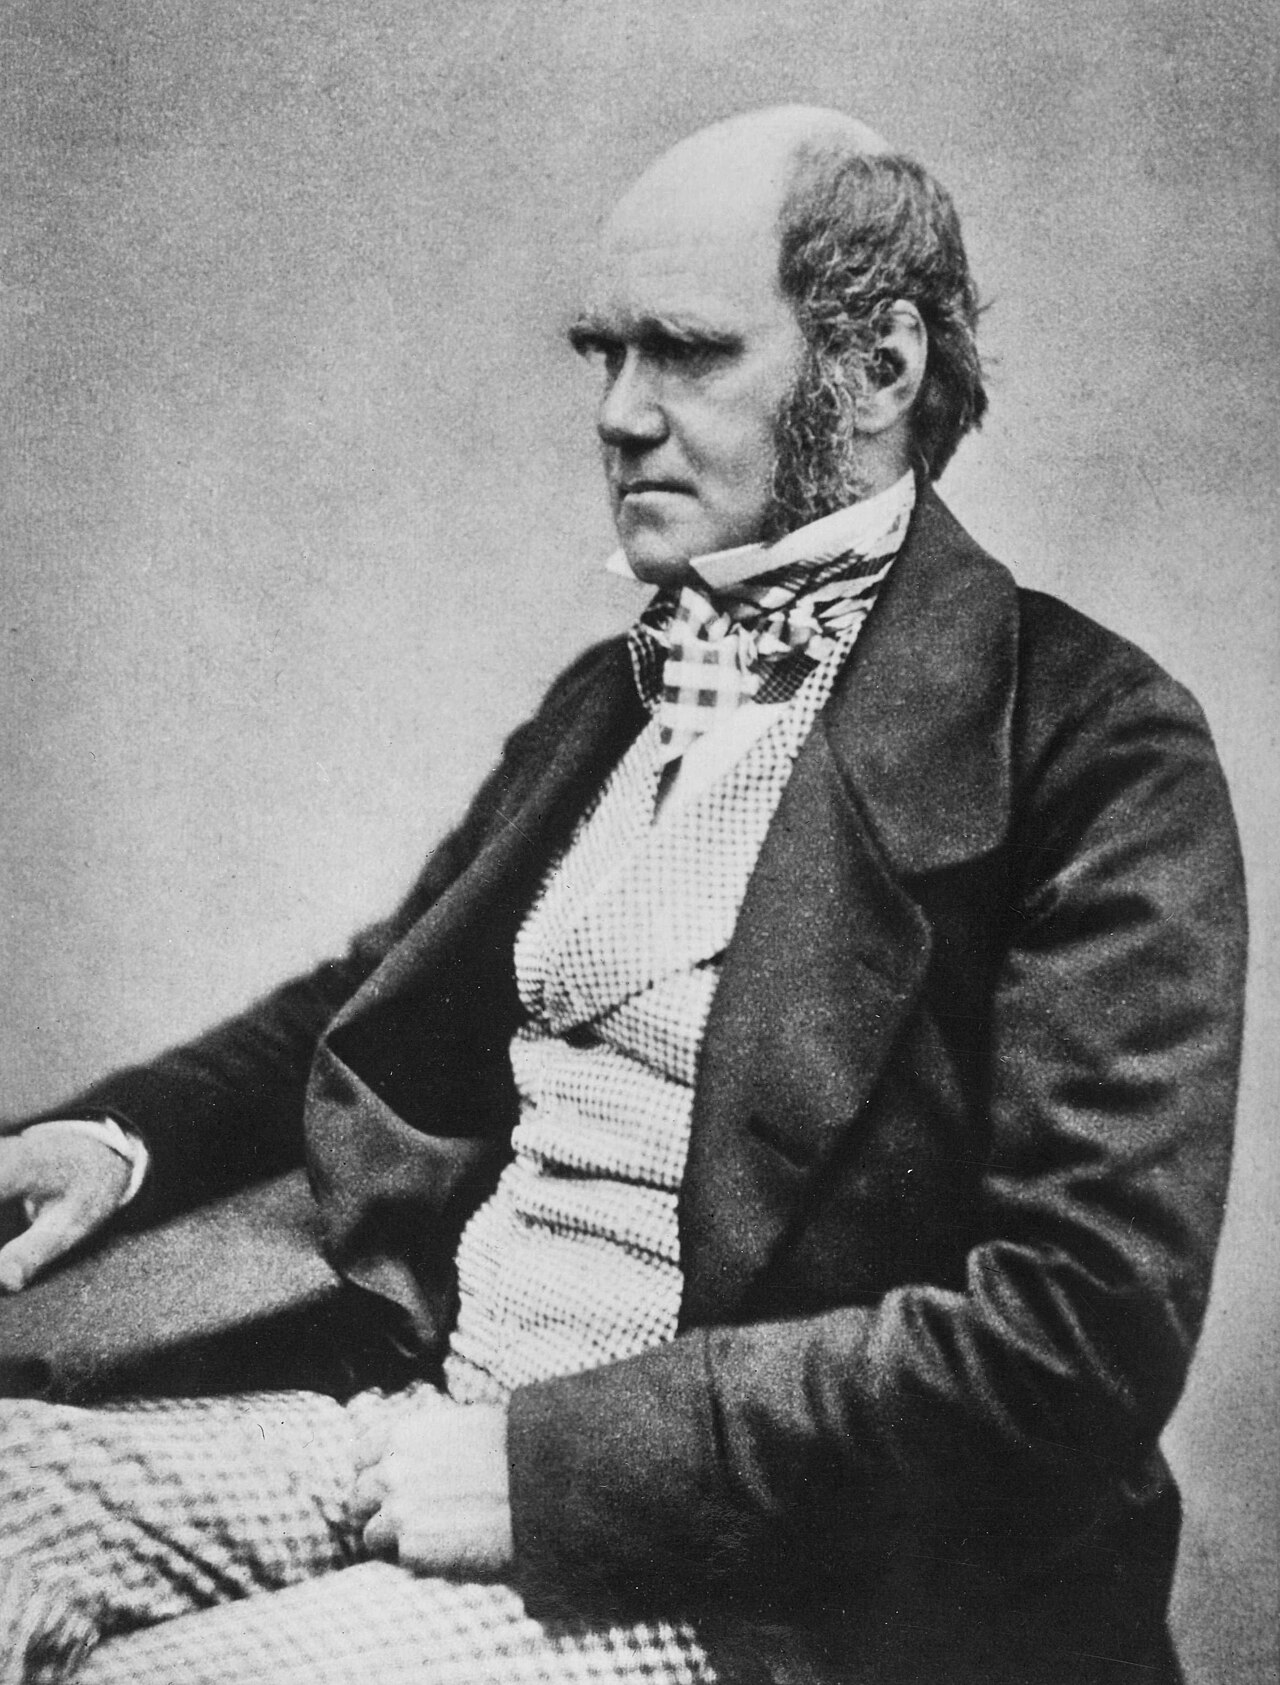
\includegraphics[width=0.36\linewidth]{images/book1/darwin.jpg}

{\small 查尔斯·达尔文，他首先将\omterm{def:g10:biodiversity-scales:species}{物种}的亲缘关系绘制成树，
并提出了使这棵树生长的机制，即\omterm{def:g12:selection-drift-speciation:selection}{自然选择}。
照片：Henry Maull and John Fox, c.~1854, 公有领域。}
\end{omfigure}

\begin{remark}[树不是什么]\label{rem:g12:phylogenetic-trees:not}
\omterm{def:g12:phylogenetic-trees:tree}{系统发生树}是关于历史的假说，由现存\omterm{def:g10:biodiversity-scales:species}{物种}构建，
并经每一新性状和每一新序列的检验；一旦两者不一致，
便需重绘，而重绘正是该领域的工作。它
没有顶端，也没有进步的方向：人类只是数以百万计的末端之一，
既不比另一末端的七鳃鳗更高等，也不更完善。
它在任何末端都没有祖先：祖先位于节点处，
已消亡的\omterm{def:g12:selection-drift-speciation:population}{种群}，其存在由树推断得出，其化石
一经发现，位于分支的旁边而非其上。
\end{remark}

\section{练习}

\begin{exercise}[$\star$]\label{exo:g12:phylogenetic-trees:1}
\omterm{def:g12:phylogenetic-trees:tree}{系统发生树}的末端、节点和根分别代表
什么？
\end{exercise}

\begin{exercise}[$\star$]\label{exo:g12:phylogenetic-trees:2}
在第一幅图的树 A 中，与蜥蜴亲缘关系最近的
是哪一\omterm{def:g10:biodiversity-scales:species}{物种}？与青蛙最近的又是哪一个？
\end{exercise}

\begin{exercise}[$\star$]\label{exo:g12:phylogenetic-trees:3}
给出共有衍生状态的定义，并说明为何共有祖先状态
不能说明亲缘关系。
\end{exercise}

\begin{exercise}[$\star$]\label{exo:g12:phylogenetic-trees:4}
什么是\omterm{prop:g12:phylogenetic-trees:rules}{演化支}？“鸟类”是\omterm{prop:g12:phylogenetic-trees:rules}{演化支}吗？“爬行动物”（取日常
含义）是\omterm{prop:g12:phylogenetic-trees:rules}{演化支}吗？
\end{exercise}

\begin{exercise}[$\star$]\label{exo:g12:phylogenetic-trees:5}
在灵长类的树中，与人类亲缘关系最近的是哪一\omterm{def:g10:biodiversity-scales:species}{物种}，
哪个节点最古老？
\end{exercise}

\begin{exercise}[$\star\star$]\label{exo:g12:phylogenetic-trees:6}
将第一幅图的树 A 重绘，使人类位于顶端，青蛙位于底端，
并检验所有亲缘关系均未改变。
\end{exercise}

\begin{exercise}[$\star\star$]\label{exo:g12:phylogenetic-trees:7}
将鸽子（颌 1，四肢 1，羊膜 1，毛发 0，羽毛 1）加入第二幅图的
矩阵中，并将其放置于树上。
性状“羽毛”提供了什么信息？
\end{exercise}

\begin{exercise}[$\star\star$]\label{exo:g12:phylogenetic-trees:8}
海豚身体呈流线型，长有类似鲨鱼的鳍，
并具有毛发、乳汁以及哺乳动物的颌。哪棵树最为简约，
这些鳍又是什么？
\end{exercise}

\begin{exercise}[$\star\star$]\label{exo:g12:phylogenetic-trees:9}
利用时钟图，推算两个\omterm{def:g10:biodiversity-scales:species}{物种}的共同祖先年代，这两个
\omterm{def:g10:biodiversity-scales:species}{物种}的 \omterm{def:g10:universal-dna:information}{DNA} 相差 2.2\%。
\end{exercise}

\begin{exercise}[$\star\star$]\label{exo:g12:phylogenetic-trees:10}
解释为什么“黑猩猩是我们的祖先”这一说法误读了
\omterm{def:g12:phylogenetic-trees:tree}{系统发生树}，并写出正确的表述。
\end{exercise}

\begin{exercise}[$\star\star$]\label{exo:g12:phylogenetic-trees:11}
在第二幅图中，为什么用七鳃鳗作为外群？
若改用小鼠，会出现什么问题？
\end{exercise}

\begin{exercise}[$\star\star\star$]\label{exo:g12:phylogenetic-trees:12}
两个\omterm{def:g10:universal-dna:gene}{基因}对三个亲缘关系很近的\omterm{def:g10:biodiversity-scales:species}{物种}给出了不同的树，这三个\omterm{def:g10:biodiversity-scales:species}{物种}
在一百万年内相继分化。解释这种情况如何能够发生，
而两棵树都不“错误”，并利用祖先\omterm{def:g12:selection-drift-speciation:population}{种群}中\omterm{def:g10:universal-dna:gene}{等位基因}的
随机混杂加以说明。
\end{exercise}

\begin{exercise}[$\star\star\star$]\label{exo:g12:phylogenetic-trees:13}
快速演化的病毒的分子钟速率为每年 1\%；
哺乳动物某\omterm{def:g10:universal-dna:gene}{基因}的分子钟速率为每百万年 0.3\%。解释为什么前者
用于追踪疫情，后者用于推定哺乳动物的起源
年代，以及为什么二者都不能承担对方的任务。
\end{exercise}

\begin{exercise}[$\star\star\star$]\label{exo:g12:phylogenetic-trees:14}
在 1.5 亿年前的岩层中发现了一种化石鸟，它长有牙齿
和细长的骨质尾巴。解释为什么它被置于\omterm{def:g12:phylogenetic-trees:tree}{系统发生树}的某一分支旁，而不是
节点上，以及它说明了该节点的什么信息。
\end{exercise}

\begin{exercise}[$\star\star\star$]\label{exo:g12:phylogenetic-trees:15}
“生命之树的顶端是人类。”请用一段话讨论，
结合读图规则、末端同龄的假设以及末端
的数目进行论述。
\end{exercise}

\section{问题：六个物种与一个分子钟}

\begin{problem}[{周末问题——分别依据性状表和 DNA 距离构建树，
比较两棵树，
并为节点定年}]
\label{pb:g12:phylogenetic-trees:1}
六个\omterm{def:g10:biodiversity-scales:species}{物种}：鲨鱼、鲑鱼、蝾螈、鳄鱼、鸽子、猫。
外群为七鳃鳗。性状表（1 为衍生状态）：

\begin{center}
\small
\begin{tabular}{lcccccc}
 & 硬骨骼 & 四肢 & 羊膜卵 & 羽毛 & 毛发 & 颅骨开口 \\ \hline
鲨鱼 & 0 & 0 & 0 & 0 & 0 & 0 \\
鲑鱼 & 1 & 0 & 0 & 0 & 0 & 0 \\
蝾螈 & 1 & 1 & 0 & 0 & 0 & 0 \\
鳄鱼 & 1 & 1 & 1 & 0 & 0 & 0 \\
鸽子 & 1 & 1 & 1 & 1 & 0 & 0 \\
猫 & 1 & 1 & 1 & 0 & 1 & 1 \\
\end{tabular}
\end{center}

某一\omterm{def:g10:universal-dna:gene}{基因}的 \omterm{def:g10:universal-dna:information}{DNA} 差异（\%）：

\begin{center}
\begin{tabular}{lccccc}
 & 鲑鱼 & 蝾螈 & 鳄鱼 & 鸽子 & 猫 \\ \hline
鲨鱼 & 30 & 31 & 30 & 31 & 30 \\
鲑鱼 & & 24 & 25 & 25 & 24 \\
蝾螈 & & & 19 & 20 & 19 \\
鳄鱼 & & & & 8 & 15 \\
鸽子 & & & & & 15 \\
\end{tabular}
\end{center}

\medskip
\noindent\textbf{第一部分——依据性状。}
\begin{enumerate}
  \item 哪一种衍生状态为最多的\omterm{def:g10:biodiversity-scales:species}{物种}所共有？写出它所定义的
        \omterm{prop:g12:phylogenetic-trees:rules}{演化支}，以及被排除在外的\omterm{def:g10:biodiversity-scales:species}{物种}。（最后一个性状是
        哺乳动物头骨侧面的单一开口，
        其为哺乳动物所具有。）
  \item 依次考察下一个共有范围最广的衍生状态，并列出
        嵌套的\omterm{prop:g12:phylogenetic-trees:rules}{演化支}。
  \item 羽毛、毛发和颅骨开口各只出现在一个\omterm{def:g10:biodiversity-scales:species}{物种}中。
        它们是否有助于构建这棵树？什么条件会使它们有用？
  \item 画出该树，在每个性状出现的
        分支上写出该性状。
  \item 根据该表，鳄鱼的最近亲缘\omterm{def:g10:biodiversity-scales:species}{物种}是哪一个？
        哪一对\omterm{def:g10:biodiversity-scales:species}{物种}仅凭该表无法确定？
\end{enumerate}

\medskip
\noindent\textbf{第二部分——依据 \omterm{def:g10:universal-dna:information}{DNA}。}
\begin{enumerate}[resume]
  \item 哪一对\omterm{def:g10:biodiversity-scales:species}{物种}的距离最小？将它们
        首先连接在一起。
  \item 下一个与该对相连的是哪个\omterm{def:g10:biodiversity-scales:species}{物种}？继续，直至
        这棵树完整为止。
  \item 比较 \omterm{def:g10:universal-dna:information}{DNA} 树与性状树：二者在何处一致，
        以及 \omterm{def:g10:universal-dna:information}{DNA} 确定了性状无法确定的哪些
        关系？
  \item 鲨鱼与其他各\omterm{def:g10:biodiversity-scales:species}{物种}的距离几乎相等。请
        根据树的形状解释原因。
  \item 鳄鱼–鸽子之间的距离（8）小于
        鳄鱼–猫之间的距离（15）。这对日常所说的
        类群“爬行动物”说明了什么？
\end{enumerate}

\medskip
\noindent\textbf{第三部分——时钟。}
化石可以确定蝾螈谱系与羊膜动物分开的时间为
340 百万年前。
\begin{enumerate}[resume]
  \item 利用蝾螈–羊膜动物之间的距离（约 19\%），计算
        时钟速率（单位为每百万年的百分之几）。（两条谱系都在变化，
        距离统计的是两条分支上发生的全部变化，
        因此两条分支都要计入。）
  \item 确定鳄鱼–鸽子节点与羊膜动物节点
        的年代（鳄鱼/鸽子与猫）。
  \item 确定鲑鱼节点与鲨鱼节点的年代。
  \item 化石表明鳄鱼–鸟类的分歧约为 250 百万年前，
        羊膜动物的分歧约为 310 百万年前。将其与你的
        年代比较，并评论单\omterm{def:g10:universal-dna:gene}{基因}时钟的准确性。
  \item 鲨鱼的距离（30--31\%）几乎不超过鲑鱼的
        （24--25\%），尽管鲨鱼节点古老得多。请提出
        一种解释，并说明这对用该\omterm{def:g10:universal-dna:gene}{基因}测定很古老节点的
        年代意味着什么。
\end{enumerate}

\medskip
\noindent\textbf{第四部分——读图与命名。}
\begin{enumerate}[resume]
  \item 按从小到大的顺序，列出你的树中包含猫的
        所有\omterm{prop:g12:phylogenetic-trees:rules}{演化支}。
  \item “鱼类”（鲨鱼与鲑鱼）是\omterm{prop:g12:phylogenetic-trees:rules}{演化支}吗？“羊膜动物”呢？请说明理由。
  \item 一名学生说蝾螈是“鱼类与爬行动物之间的中间类型”。
        请用树的术语改正这一说法。
  \item 发现一块化石，具有骨质骨骼、四肢，且没有羊膜卵，
        年代为 360 百万年。它在树上处于什么位置？其年代
        证实了什么？
  \item 给出结论：六个\omterm{def:g10:biodiversity-scales:species}{物种}的树（写成嵌套括号的形式）、
        \omterm{def:g10:universal-dna:information}{DNA} 确定的唯一亲缘关系，
        以及鳄鱼–鸽子分歧的估计年代。
\end{enumerate}
\end{problem}
